%!TEX ROOT=../ctutest.tex

\chapter{Dissertation plan}
\label{chap:plan}


\section{Current research agenda}
\subsection{Automated claim generation}
\todo{}
\subsection{Claim generation metrics}

\begin{figure}
    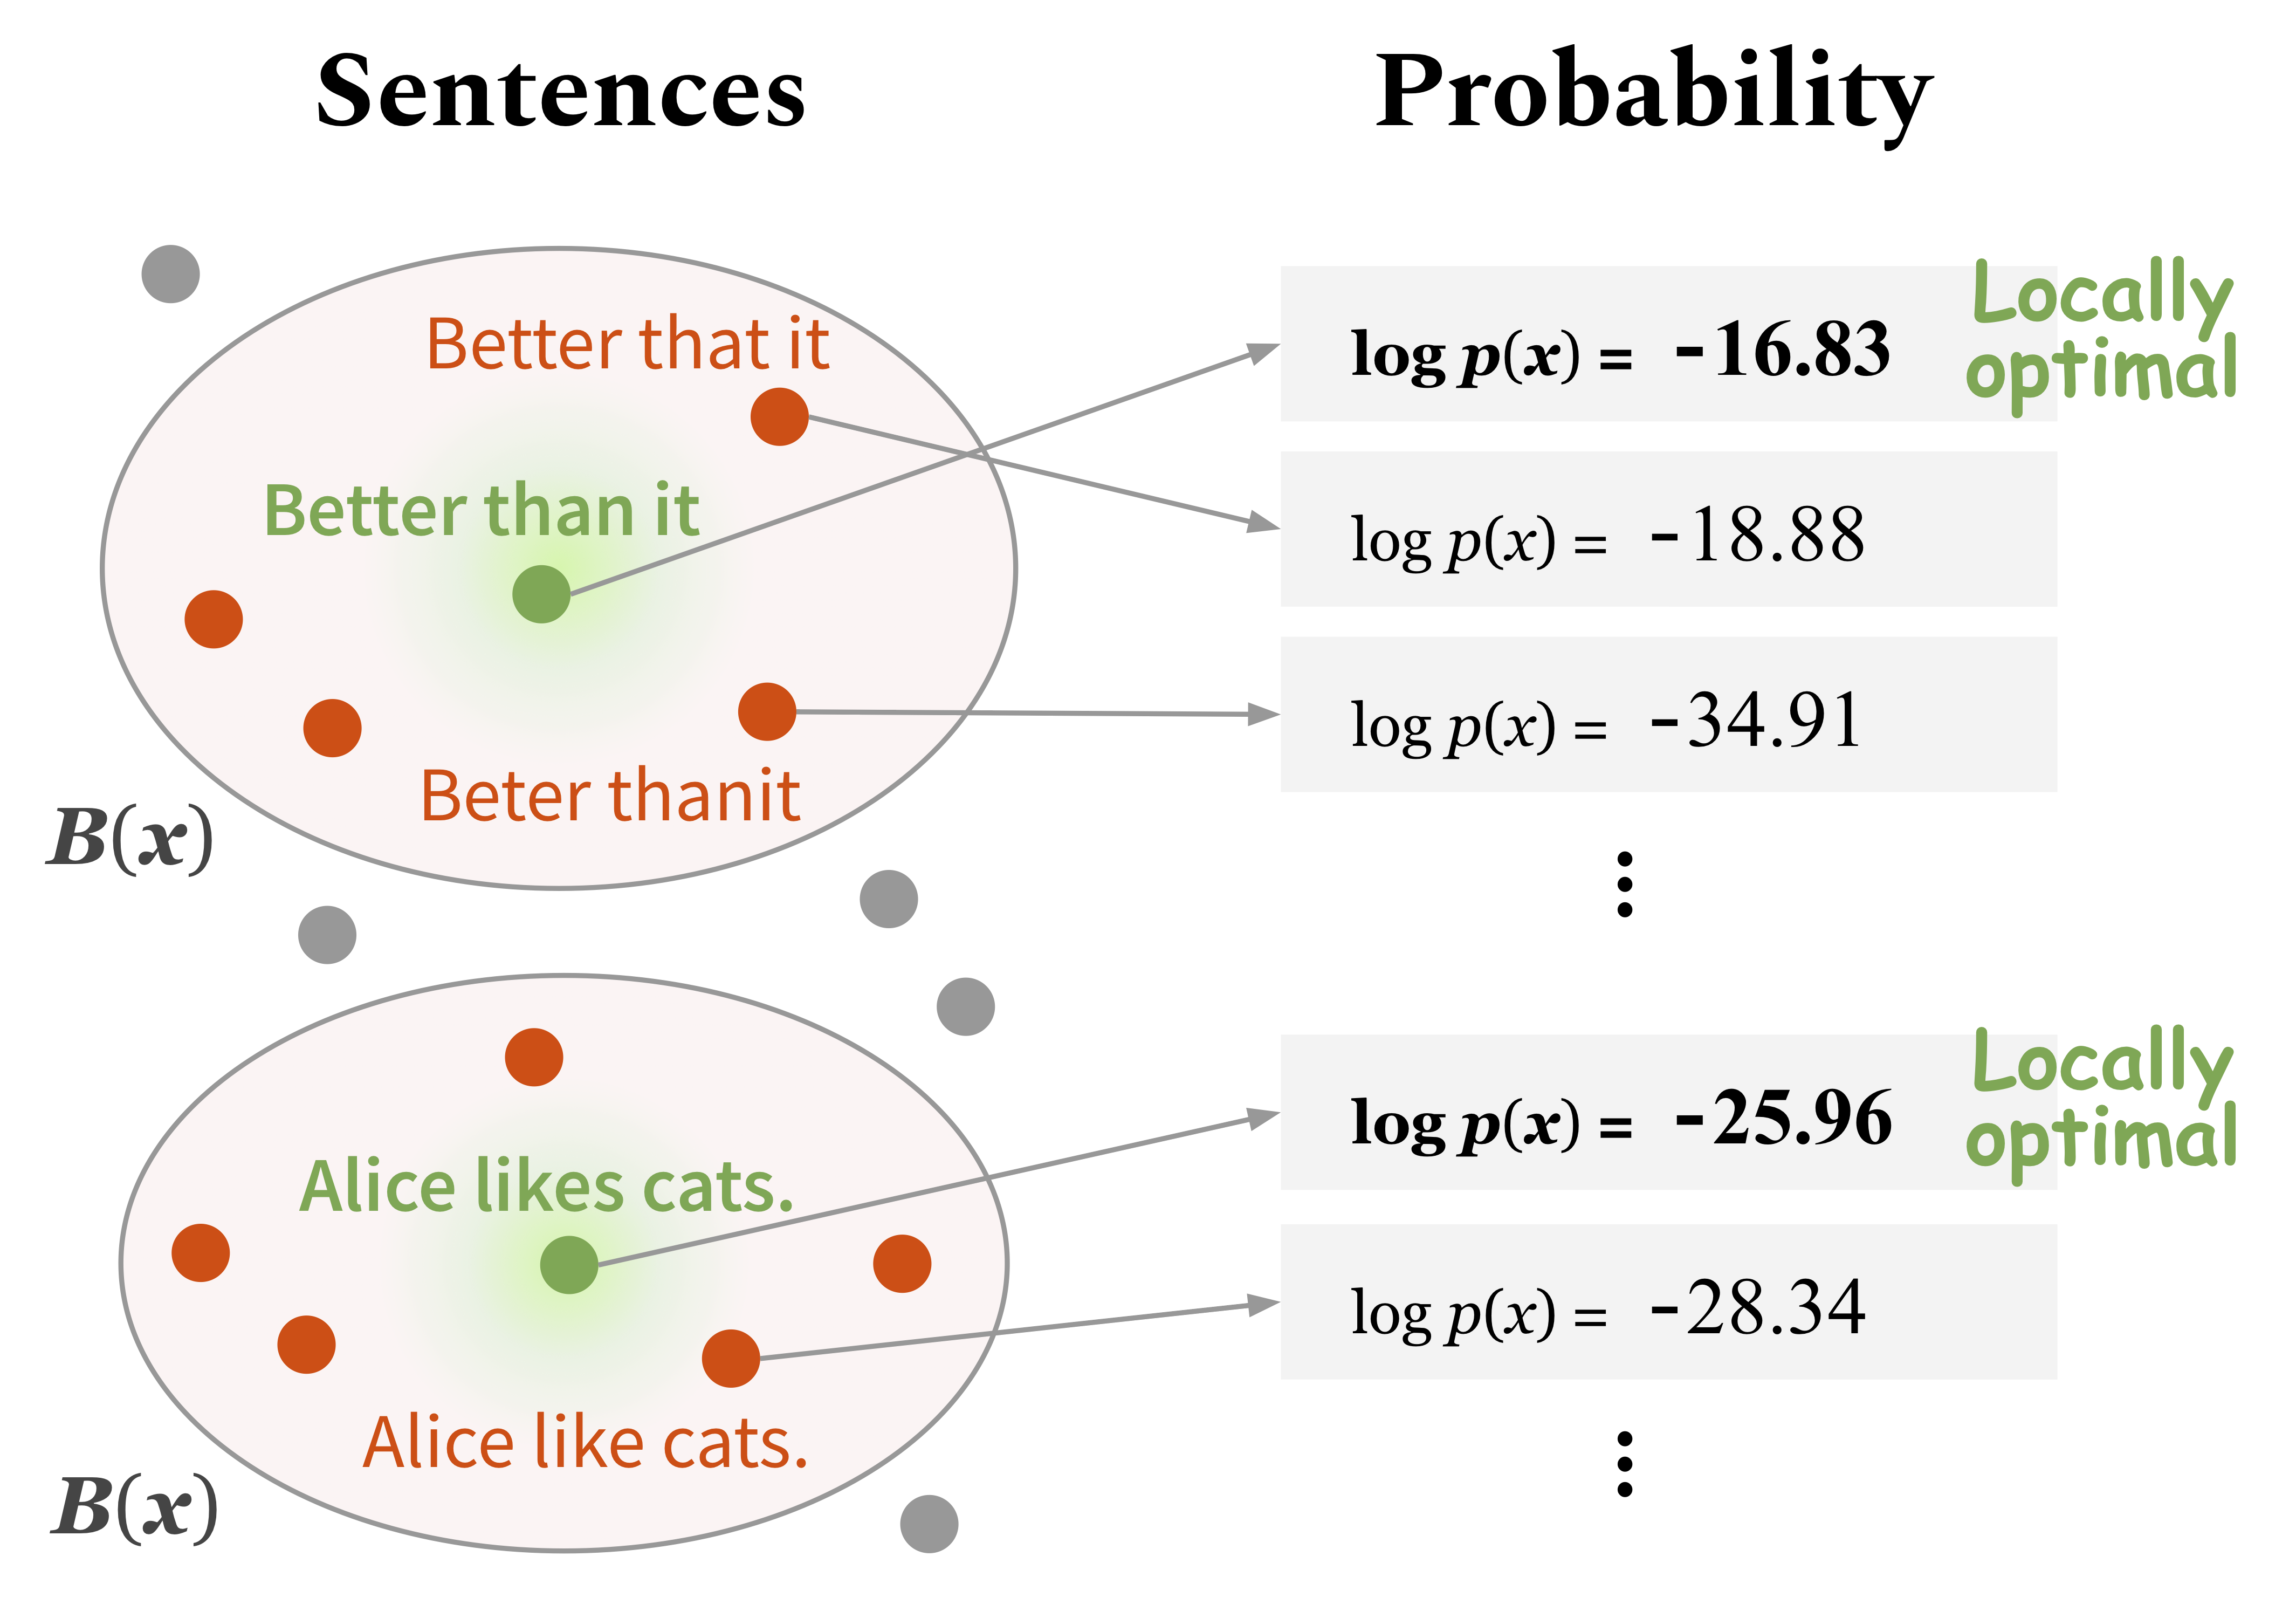
\includegraphics[width=7cm]{fig/lm_critics.png}
    \caption{\textsf{LM-Critic} -- deciding text fluency viewed as finding local optima of Language Model output probability, reprinted from~\cite{yasunaga-etal-2021-lm}}
    \label{fig:gptext}
\end{figure}
\label{sec:metrics}

\begin{figure}
    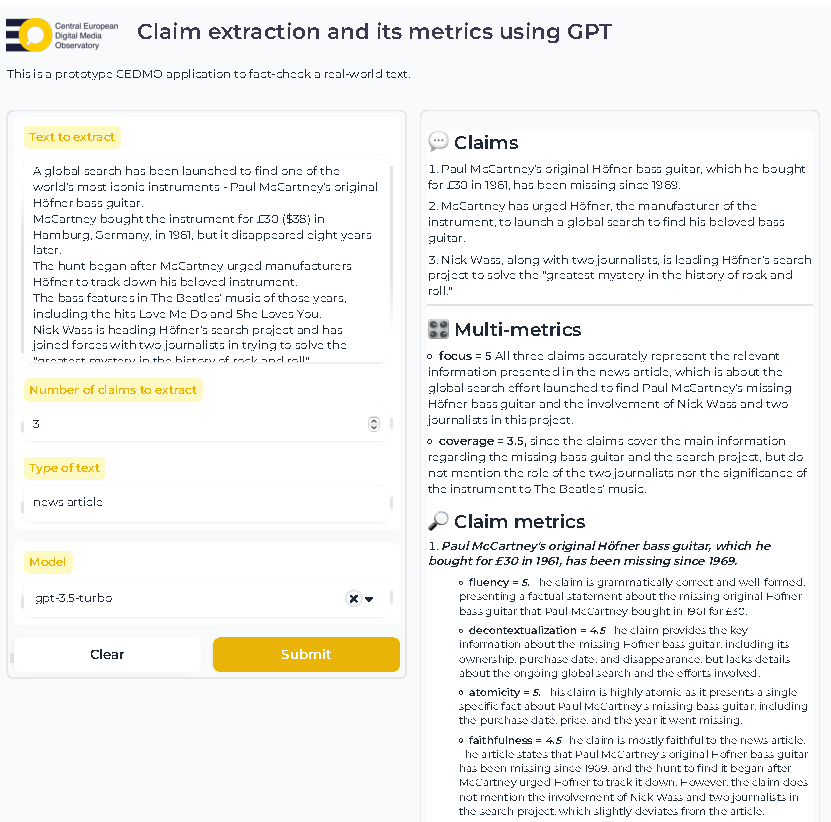
\includegraphics[width=11cm]{fig/gptext.pdf}
    \caption{A self-evaluating claim generation model based on GPT-4~\cite{gpt4} using the \textsf{OpenAI API} and a few-shot approach}
    \label{fig:gptext}
\end{figure}
\label{sec:metrics}
The common problem with generative tasks in NLP is that of explaining their reasoning in human-understandable manner and troubleshooting the prediction faults, such as the \textit{model hallucination}.

For the task of claim generation, where we also face the challenge of the \textit{relevance} of the information extracted by the model, we postulate the following metrics:

\begin{enumerate}
    \item {\techbf Fluency} -- \textit{is the claim grammatically correct and intelligible?}
    
    Currently, we are working with two emulations of claim fluency, task that is similar to a standard NLP task of Gramatical Error Detection (GED): \textsf{LM-Critic} (Figure)~\cite{yasunaga-etal-2021-lm} perturbs the claim words and characters to find local optima in output probability of its tokens, using a language model such as GPT-2 as its reference. \textsf{GPTScore}~\cite{fu2023gptscore} uses prompting a LLM (such as GPT-3.5) to obtain a model-inferred score using zero-shot learning.
    
    Both can be adapted for Czech and the latter is demonstrated in Figure~\ref{fig:gptext}.
    \item {\techbf Decontextualization} -- \textit{can the claim be correctly interpreted without any additional context from the source document or elsewhere?}\\
    \todo{Making sentences stand alone}
    \item {\techbf Atomicity} --  \textit{does the claim describe a single entity, relation or process?}
    
    can be checked using the Relationship Extraction methods such as LUKE~\cite{yamada2020luke}. To put it simply, the RE task is to identify the entities of a text (persons, institutions,\dots) and the relations between them (such as $(\textit{\"{study at}}, \textit{Herbert}, \textit{CTU})$). The atomicity evaluation can be converted to a RE task by attempting to extract such fact triples and mark the claim as atomic if there is at most one such triple to extract (after removing symmetries)
    \item {\techbf Faithfulness} -- \textit{does the claim only contain information that follows from the source document?}
    
    This metric is crucial to pinpoint \textit{model hallucinations} -- parts of claim where the model outputs stray from the information present in source text and begin to just \"{make stuff up}. We proceed to use two alternative metrics -- a score proposed within the FFCI evaluation framework~\cite{ffci} as: 
    $$AvgTopN(BERTScore(t_i,s_j))$$
    Similar metric was proposed in~\cite{zha2023alignscore}, looking for optimum alignment of output and parts of input, using an arbitrary 
    \item {\techbf Focus}$@k$ -- \textit{if we generate $k$ claims using this model, what will be the proportion of gold (relevant) information among all the information listed in the generated claims?}\\
    we use the question-answering-based solutions of QAGS~\cite{wang-etal-2020-asking}
    \item {\techbf Coverage}$@k$ -- \textit{if we generate $k$ claims using this model, what proportion of gold (relevant) information from the source text will be covered?}\\
    we use the question-answering-based solutions of QAGS~\cite{wang-etal-2020-asking}
\end{enumerate}

\section{Data Collection}
\subsection{Human-in-the-loop grading of claim generators}
\subsection{Validation of the model outputs with human fact-checkers}
\subsection{Polish dataset scraping}
Will be first of its kind for NLP purposes

\subsection{Crowd-sourced fact checking platform}
\todo{Cite boys}~\cite{butora}
\section{The grand scope}
\begin{enumerate}
    \item \textbf{Claim extraction metrics proposal based on factuality of summarization}
    \item \textbf{Claim extraction paradigm that benchmarks best in the newly given metrics}
    \item Systems for NLI built on top of LoRA paradigm to score best in the task, as showed promising by Daniil
    
\end{enumerate}